\documentclass[11pt,fleqn]{article}
\usepackage[letterpaper]{geometry}
\usepackage{graphicx}    % needed for including graphics e.g. EPS, PS
\usepackage{amsmath}
\usepackage{xfrac}
\usepackage[version=4]{mhchem}
\usepackage{listings}
\usepackage{hyperref}
\usepackage{wrapfig}
\usepackage{empheq}
\usepackage{capt-of}



% To use UTF-8 characters
\usepackage[utf8x]{inputenc}
% \DeclareUnicodeCharacter{207A}{$^+$}
% \DeclareUnicodeCharacter{207B}{$^-$}







% color def PYTHON CODE
\usepackage{color}
\definecolor{darkred}{rgb}{0.6,0.0,0.0}
\definecolor{darkgreen}{rgb}{0,0.50,0}
\definecolor{lightblue}{rgb}{0.0,0.42,0.91}
\definecolor{orange}{rgb}{0.99,0.48,0.13}
\definecolor{grass}{rgb}{0.18,0.80,0.18}
\definecolor{pink}{rgb}{0.97,0.15,0.45}

% listings
\usepackage{listings}

% General Setting of listings
\lstset{
	aboveskip=1em,
	breaklines=true,
	abovecaptionskip=-6pt,
	captionpos=b,
	escapeinside={\%*}{*)},
	frame=single,
	numbers=left,
	numbersep=15pt,
	numberstyle=\tiny,
}
% 0. Basic Color Theme
\lstdefinestyle{colored}{ %
	basicstyle=\ttfamily,
	backgroundcolor=\color{white},
	commentstyle=\color{green}\itshape,
	keywordstyle=\color{blue}\bfseries\itshape,
	stringstyle=\color{red},
}
% 1. General Python Keywords List
\lstdefinelanguage{PythonPlus}[]{Python}{
	morekeywords=[1]{,as,assert,nonlocal,with,yield,self,True,False,None,} % Python builtin
	morekeywords=[2]{,__init__,__add__,__mul__,__div__,__sub__,__call__,__getitem__,__setitem__,__eq__,__ne__,__nonzero__,__rmul__,__radd__,__repr__,__str__,__get__,__truediv__,__pow__,__name__,__future__,__all__,}, % magic methods
	morekeywords=[3]{,object,type,isinstance,copy,deepcopy,zip,enumerate,reversed,list,set,len,dict,tuple,range,xrange,append,execfile,real,imag,reduce,str,repr,}, % common functions
	morekeywords=[4]{,Exception,NameError,IndexError,SyntaxError,TypeError,ValueError,OverflowError,ZeroDivisionError,}, % errors
	morekeywords=[5]{,ode,fsolve,sqrt,exp,sin,cos,arctan,arctan2,arccos,pi, array,norm,solve,dot,arange,isscalar,max,sum,flatten,shape,reshape,find,any,all,abs,plot,linspace,legend,quad,polyval,polyfit,hstack,concatenate,vstack,column_stack,empty,zeros,ones,rand,vander,grid,pcolor,eig,eigs,eigvals,svd,qr,tan,det,logspace,roll,min,mean,cumsum,cumprod,diff,vectorize,lstsq,cla,eye,xlabel,ylabel,squeeze,}, % numpy / math
}
% 2. New Language based on Python
\lstdefinelanguage{PyBrIM}[]{PythonPlus}{
	emph={d,E,a,Fc28,Fy,Fu,D,des,supplier,Material,Rectangle,PyElmt},
}
% 3. Extended theme
\lstdefinestyle{colorEX}{
	basicstyle=\ttfamily,
	backgroundcolor=\color{white},
	commentstyle=\color{darkgreen}\slshape,
	keywordstyle=\color{blue}\bfseries\itshape,
	keywordstyle=[2]\color{blue}\bfseries,
	keywordstyle=[3]\color{grass},
	keywordstyle=[4]\color{red},
	keywordstyle=[5]\color{orange},
	stringstyle=\color{darkred},
	emphstyle=\color{pink}\underbar,
}









\usepackage{tikz}
\usepackage{tikzpagenodes}
\usetikzlibrary{positioning}

\topmargin -1.5cm        % read Lamport p.163
\oddsidemargin -0.04cm   % read Lamport p.163
\evensidemargin -0.04cm  % same as oddsidemargin but for left-hand pages
%\textwidth 16.59cm
\textwidth 11cm
\textheight 21.94cm 
%\pagestyle{empty}       % Uncomment if don't want page numbers
\parskip 7.2pt           % sets spacing between paragraphs
%\renewcommand{\baselinestretch}{1.5} 	% Uncomment for 1.5 spacing between lines
\parindent 0pt		  % sets leading space for paragraphs


\newcounter{qNum}
\newcommand{\qn}{\refstepcounter{qNum} \theqNum}
\newcounter{qNumH}
\newcommand{\qnH}{\refstepcounter{qNumH}  \textit{Honors} \theqNumH}
\newcommand{\eqn}{\text{\qn) \ }}
\def \dt {\ensuremath{\,\mathrm{d}t}}

\newcommand{\aspace}{ \hspace{1em}\\ \vspace{8em}}

\newcommand{\dx}{\; dx}

\newcommand{\D}[1]{\; d{#1}}

\newcommand{\graphGrid}{
	
\begin{tikzpicture}
	\draw[step=.5cm,gray,help lines] (-5,-5) grid (5,5);
	\draw[step=2.5cm,black,very thin] (-5,-5) grid (5,5);
	\end{tikzpicture}
}

\newcommand{\graphGridAxes}{
	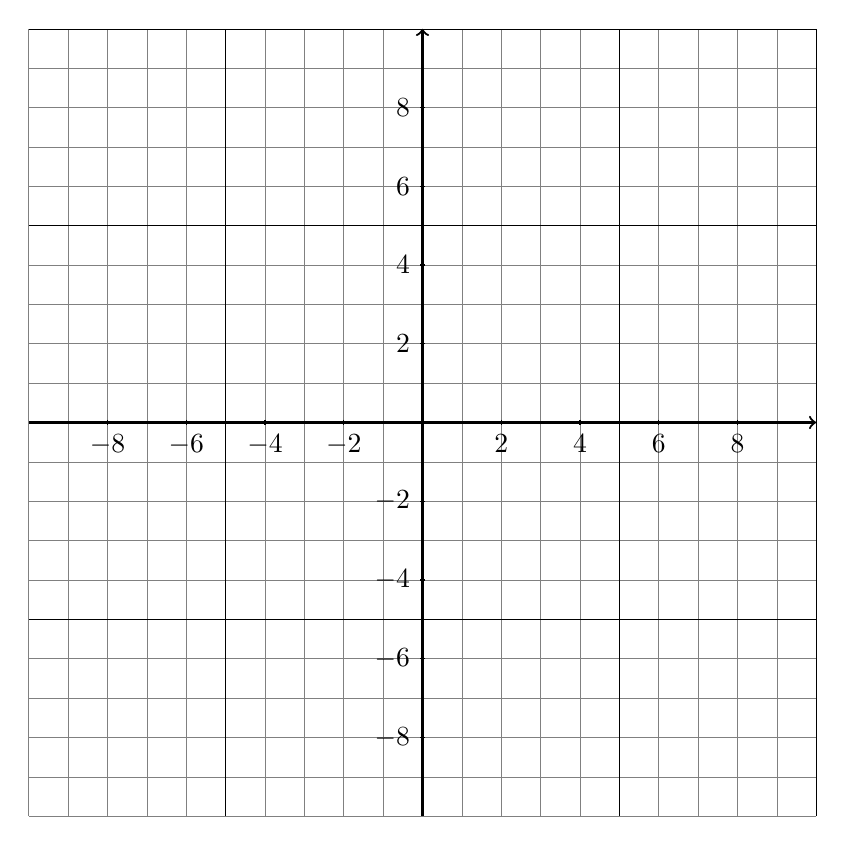
\begin{tikzpicture}
	\draw[step=.5cm,gray,help lines] (-5,-5) grid (5,5);
	\draw[step=2.5cm,black,very thin] (-5,-5) grid (5,5);
	\draw[thick,->] (-5,0) -- (5,0) ;
	\draw[thick,->] (0,-5) -- (0,5) ; 
	\foreach \x in {-8, -6, -4, -2,  2,4, 6, 8}
	\draw (\x*0.5 cm,1pt) -- (\x*0.5 cm,-1pt) node[anchor=north] {$\x$};
	\foreach \y in {-8, -6, -4, -2,  2,4, 6, 8}
	\draw (1pt,\y*0.5 cm) -- (-1pt,\y*0.5 cm) node[anchor=east] {$\y$};
	\end{tikzpicture}
}

\newcommand{\graphGridAxesS}[1]{
	\begin{tikzpicture}
		\draw[step=.5cm,gray,help lines] (-0.5*#1,-0.5*#1) grid (0.5*#1, 0.5*#1);
		\draw[step=2.5cm,black,very thin] (-0.5*#1,-0.5*#1) grid (0.5*#1, 0.5*#1);
		\draw[thick,->] (-#1/2,0) -- (#1/2,0) ;
		\draw[thick,->] (0,-#1/2) -- (0,#1/2) ; 
		\foreach \x in {-8, -6, -4, -2,  2,4, 6, 8}
		\draw (\x*0.5 cm,1pt) -- (\x*0.5 cm,-1pt) node[anchor=north] {$\x$};
		\foreach \y in {-8, -6, -4, -2,  2,4, 6, 8}
		\draw (1pt,\y*0.5 cm) -- (-1pt,\y*0.5 cm) node[anchor=east] {$\y$};
	\end{tikzpicture}
}



%headers
\usepackage{datetime}
\usepackage{fancyhdr}
\pagestyle{fancy}
\lhead{ Name: }
\rhead{\footnotesize Finite Difference Method: Cylindrical Tube (\monthname, \the\year)}
\title{Introduction to the Finite Difference Method: \\ Draining a Cylindrical Tube}
\author{Lensyl Urbano}



 \begin{document}         
 % Start your text
 
\maketitle
Consider a cylinder with water draining out of the bottom through a hole.
	\begin{tikzpicture}[remember picture,overlay,shift={(current page.east)}]
	\node[anchor=north east,xshift=-2cm](myImage){
		%\centering
		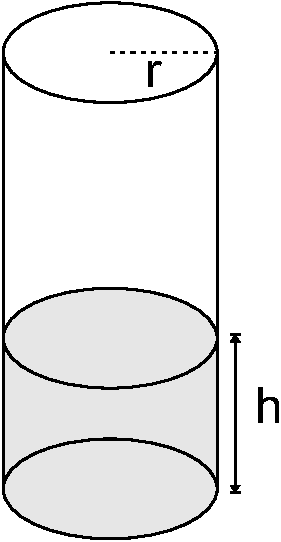
\includegraphics[height=5cm]{cylinder-rh.pdf} 
	};
	\node[inner sep=0pt,text width=0.5\linewidth] (myCaption) [below=of myImage]
	{\captionof{figure}{Cylinder with dimensions. $r$ is the radius and $h$ is the height of water in the tube.}};
\end{tikzpicture}

\section{Numerical Solution}

	For draining, the outflow rate (change in volume over time, ($Q=\frac{dV}{dt}$) is not constant. The outflow rate is proportional to the height of water in the tube, since the higher the water level the greater pressure at the bottom of the tube and the faster the outflow rate.
	\begin{equation}
		\frac{dV}{dt} \propto h
	\end{equation}
	
	Converting the proportionality statement to an equation requires us to introduce a constant ($k$):
	\begin{equation}
		\label{eqn:flowRate}
		\frac{dV}{dt} = k \cdot h
	\end{equation}
	
	As we saw when we were filling the cylinder, the change in height of water in the tube is given by the \textbf{change in height} equation:
	\begin{empheq}[box=\fbox]{equation}
		\label{eqn:dh_eqn}
		\Delta h = \frac{\Delta t}{\pi r^2} \; Q 
	\end{empheq}
	
	where $Q$ is $\frac{dV}{dt}$ so:
	\begin{equation}
		\Delta h = \frac{\Delta t}{\pi r^2} \; \frac{dV}{dt}
	\end{equation}
	
	So, let's substitute our flow rate equation (Eqn. \ref{eqn:flowRate}) for $\frac{dV}{dt}$ to get:
	\begin{empheq}[]{equation}
		\Delta h = \frac{\Delta t}{\pi r^2} \; k \cdot h
	\end{empheq}
	
	Important to note for the computer model, is that the height ($h$) used in this equation is the old height from the previous timestep so:
	\begin{empheq}[box=\fbox]{equation}
		\Delta h = \frac{\Delta t}{\pi r^2} \; k \cdot h_{old}
	\end{empheq}

	and we can still update the new height using:
	\begin{empheq}[box=\fbox]{equation}
		\label{eqn:hnew_eqn}
		h_{new} = h_{old} + \Delta h
	\end{empheq}
	
	so, in our code we just need to change this line and set up a few different constants.



\subsection{Code: Draining}

	This program is based off the filling code, but for this example we ignore the filling by setting the inflow rate to zero (\textbf{Line 12}). We're using an initial height of 50 cm ($h_0 = 50$), and set the constant $k$ to be equal to one. 

	\textit{water-draining-fd.py}
	\begin{tikzpicture}[remember picture,overlay,shift={(current page.east)}]
		\node[anchor=north east,xshift=-1cm](myImage){
			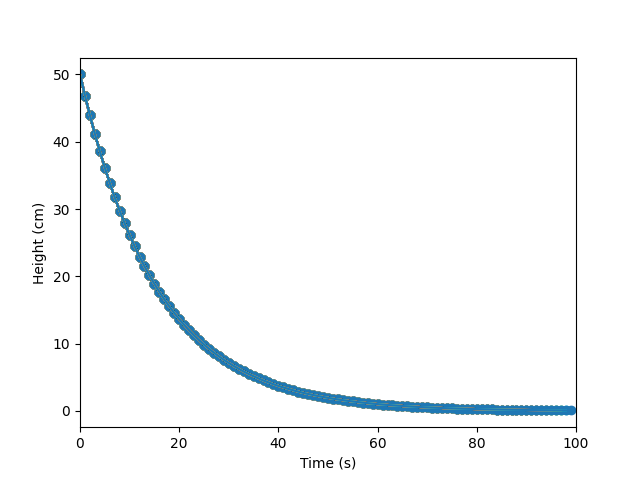
\includegraphics[height=5cm]{water-draining-fd.png} 
		};
		\node[inner sep=0pt,text width=0.5\linewidth] (myCaption) [below=of myImage]
		{\captionof{figure}{\label{drainingModel} Model output: Graph of height of water in the column over time when draining the cylinder via a hole in the bottom.  }};
	\end{tikzpicture}
	
	\lstinputlisting[language=Python, frame=single]{../water-draining-fd.py}
	

The output from the model (Fig. \ref{drainingModel}) looks like an exponential decay curve, which is what we will find from the analytical solution (Eqn. \ref{analyticalDraining}).



\section{Draining: Analytical Solution using Calculus}
	Experiments (which you may have done) show that if you're draining a cylinder by gravity the outflow rate of water is linearly proportional to the height of water in the tube. 
	\begin{equation}
		\frac{dV}{dt} \propto h
	\end{equation}

	Converting the proportionality statement to an equation requires us to introduce a constant ($k$):
	\begin{equation}
		\label{DrainingDiffEqn}
		\frac{dV}{dt} = k h
	\end{equation}

	So in draining, the outflow rate ($\frac{dV}{dt}$) is not constant, it slows down as the height of water in the tube decreases. 
	
	Now, lets substitute the equation for the volume of a cylinder:
	\begin{equation}
		V = \pi r^2 h
	\end{equation}
	
	into the draining equation (Eq. \ref{DrainingDiffEqn}) to get:
	\begin{equation}
		\frac{d[\pi r^2 h]}{dt} = k h
	\end{equation}

	we can extract $\pi$ and $r^2$ from the differential because they are constant:
	\begin{equation}
		\pi r^2 \frac{dh}{dt} = k h
	\end{equation}

	separating the variables gives:
	\begin{equation}
		\pi r^2 \frac{dh}{h} = k \cdot dt
	\end{equation}
	and rearranging:
	\begin{equation}
		\frac{dh}{h} = \frac{k \cdot dt}{\pi r^2 }
	\end{equation}
	\begin{equation}
		\frac{dh}{h} = \frac{k}{\pi r^2 } dt
	\end{equation}

	To simplify a little, lets consolidate the constants on the left hand side into one variable $K$:
	\begin{equation}
		K = \frac{k}{\pi r^2 }
	\end{equation}
	so:
	\begin{equation}
		\frac{dh}{h} = K \cdot dt 
	\end{equation}
	
	which we can integrate (remember $K$ is a constant):
	\begin{align}
		\int \frac{dh}{h} &= K \int dt \\
		\ln{h} &= K \cdot t + c
	\end{align}
	
	we can solve for $h$ by raising both sides by $e$ to cancel the $\ln$:
	\begin{equation}
		e^{\ln{h}} = e^{K t + c}
	\end{equation}

	\begin{equation}
		h = e^{K t + c}
	\end{equation}

	Because of math, we can pull the constant out to get:
	\begin{equation}
		h = Ce^{K t}
	\end{equation}

	Where the constant is the initial value of the height ($h_0$):
	\begin{empheq}[]{equation}
		\label{analyticalDraining}
		h = h_0 \cdot e^{K t}
	\end{empheq}

	This is an exponential function. If $K$ is less than 1 ($K<1$) then this is a decay curve.
	
	

 % Stop your text
 \end{document}
